\section{Implementation}

In this section will be presented simple $C\#$ program as an example implementation of presented topics.
By design it implements the simplest multilayer network with two inputs and one output to model boolean functions.
Program is capable to learn non linearly separable XOR function and show this process.

\subsection{User interface}

User interface presents the network structure.

\begin{figure}[!h]
    \centering
    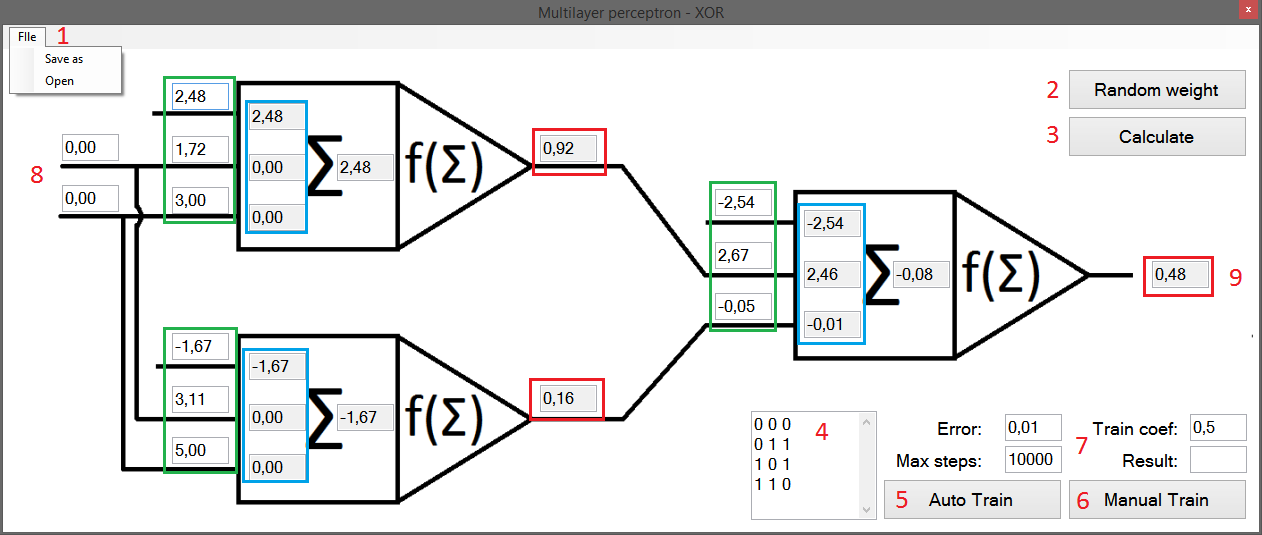
\includegraphics[scale=0.45]{Media/UI_numbers.png}
    \caption{User interface}
    \label{fig:UI}
\end{figure}

